%==============================================================================
\chapter{Electrical specifications}
%------------------------------------------------------------------------------
\section{Pad layout}

Fig.~\ref{fig:ROCpadschematic} shows the main wire-bond pads and their names. 

\begin{figure}[hbtp]
	\begin{center}
	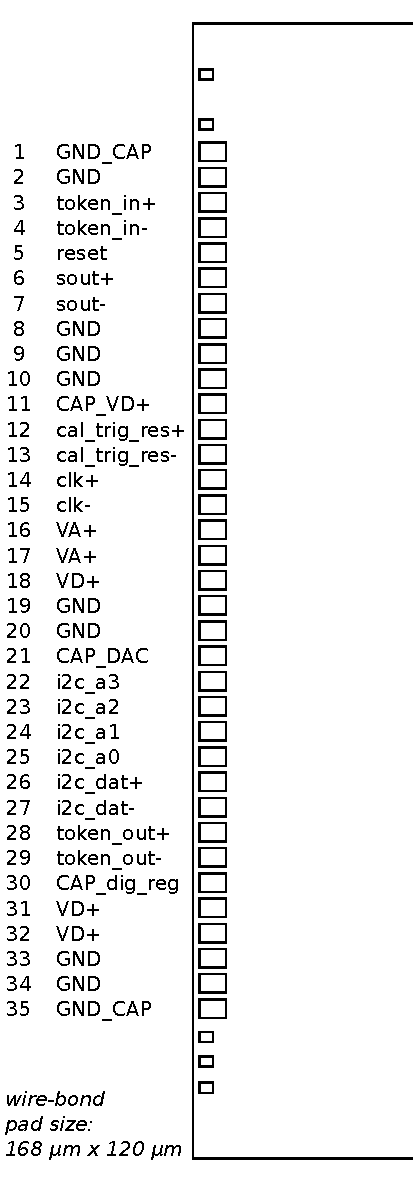
\includegraphics[width=.3\textwidth]{img/ROC_padschema.pdf}
	\end{center}
	\caption{Location and names of wire-bond pads on the chip. The pitch of the wirebond pads is 175\,$\mu$m.}
	\label{fig:ROCpadschematic}
\end{figure}

%------------------------------------------------------------------------------
\section{Powering and signals}
Table~\ref{tab:ROCpinout} describes the meaning of the signals. 
\begin{table}[h]
    \begin{center}
	\caption{\textbf{List of wire-bond pads.} }
	\label{tab:ROCpinout}

	\bigskip

	{\scriptsize
	\begin{tabular}{clcl}
	\toprule %-------------------------------------------------------------------------------------------------
	Pin\# & Name         & Type & Description \\
	\midrule %-------------------------------------------------------------------------------------------------
	 1 & GND\_CAP        & out & External filter capacitances, connected to GND internally in the chip \\
	\midrule %-------------------------------------------------------------------------------------------------
	 2 & GND             & in  & Ground \\
	\midrule %-------------------------------------------------------------------------------------------------
	 3 & token\_in+      & in  & \multirow{2}{*}{Readout token} \\
	 4 & token\_in-      & in  & \\
	\midrule %-------------------------------------------------------------------------------------------------
	 5 & reset           & in  & Hard chip reset, resets all double columns, \isqc{}, DAC's \\
	\midrule %-------------------------------------------------------------------------------------------------
	 6 & sout+           & out & \multirow{2}{*}{Serial output of data} \\
	 7 & sout-           & out & \\
	\midrule %-------------------------------------------------------------------------------------------------
	 8 & GND             & in  & \multirow{3}{*}{Ground}  \\
	 9 & GND             & in  & \\
	10 & GND             & in  & \\
	\midrule %-------------------------------------------------------------------------------------------------
	11 & CAP\_VD+        & out & External capacity filtering unregulated VD, internally connected to pad 18 \\
	\midrule %-------------------------------------------------------------------------------------------------
	12 & cal\_trig\_res+ & in  & \multirow{2}{*}{Combined signal: calibrate/trigger/reset} \\
	13 & cal\_trig\_res- & in  & \\
	\midrule %-------------------------------------------------------------------------------------------------
	14 & clk+            & in  & \multirow{2}{*}{40\,MHz clock} \\
	15 & clk-            & in  & \\
	\midrule %-------------------------------------------------------------------------------------------------
	16 & VA+             & in  &\multirow{2}{*}{Analog voltage +1.5\,V} \\
	17 & VA-             & in  & \\
	\midrule %-------------------------------------------------------------------------------------------------
	18 & VC+             & in  & Input to supply the comparators with +2.5\,V (same as VD+), see also pad 11 \\
	\midrule %-------------------------------------------------------------------------------------------------
	19 & GND             & in  & \multirow{2}{*}{Ground} \\
	20 & GND             & in  & \\
	\midrule %-------------------------------------------------------------------------------------------------
	21 & CAP\_DAC        & out & External capacity filtering the internally regulated voltage supplying th DAC's \\
	\midrule %-------------------------------------------------------------------------------------------------
	22 & i2c\_a3         & in  & \multirow{4}{*}{Chip address bits 0 to 3} \\
	23 & i2c\_a2         & in  & \\
	24 & i2c\_a1         & in  & \\
	25 & i2c\_a0         & in  & \\
	\midrule %-------------------------------------------------------------------------------------------------
	26 & i2c\_dat+       & in  & \multirow{2}{*}{\isqc{} data SDA} \\
	27 & i2c\_dat-       & in  & \\
	\midrule %-------------------------------------------------------------------------------------------------
	28 & token\_out+     & out & \multirow{2}{*}{Readout token output} \\
	29 & token\_out-     & out & \\
	\midrule %-------------------------------------------------------------------------------------------------
	30 & CAP\_dig\_reg   & out & External capacitance filtering VD regulated \\
	\midrule %-------------------------------------------------------------------------------------------------
	31 & VD+             & in  & \multirow{2}{*}{Digital voltage +2.5\,V} \\
	32 & VD-             & in  & \\
	\midrule %-------------------------------------------------------------------------------------------------
	33 & GND             & in  & \multirow{2}{*}{Ground}\\
	34 & GND             & in  & \\
	\midrule %-------------------------------------------------------------------------------------------------
	35 & GND\_CAP        & out & External filter capacitances, connected to GND internally in the chip \\
	\bottomrule %-------------------------------------------------------------------------------------------------
	\end{tabular}
	}
    \end{center}
\end{table}
